\chapter{Conclusions, Limitations, and Future Work (Work in Progress)}
\label{chp:conclusions}

\section{Summary of dissertation.}

\subsection{Perspective and Significance of Research}
This dissertation has presented data centers from my perspectives as a facilities designer, hardware deployment engineer, and resource capacity manager. The data center form-factors I reason about through out this work are the hyper-scale data center campuses that are used for global platforms; such as search engines, social media, and public cloud services. These data centers are a critical components of the modern day lives of people, yet by design they are generally hidden from the public view. An example of the hidden critically of DCs is the on-going stay-in-place orders; in which remote work and school over-the-internet has become a normal way of life for many across the world. 

\usepackage{rotating}
\begin{sidewaysfigure}
% \begin{figure}[h!]\centering
    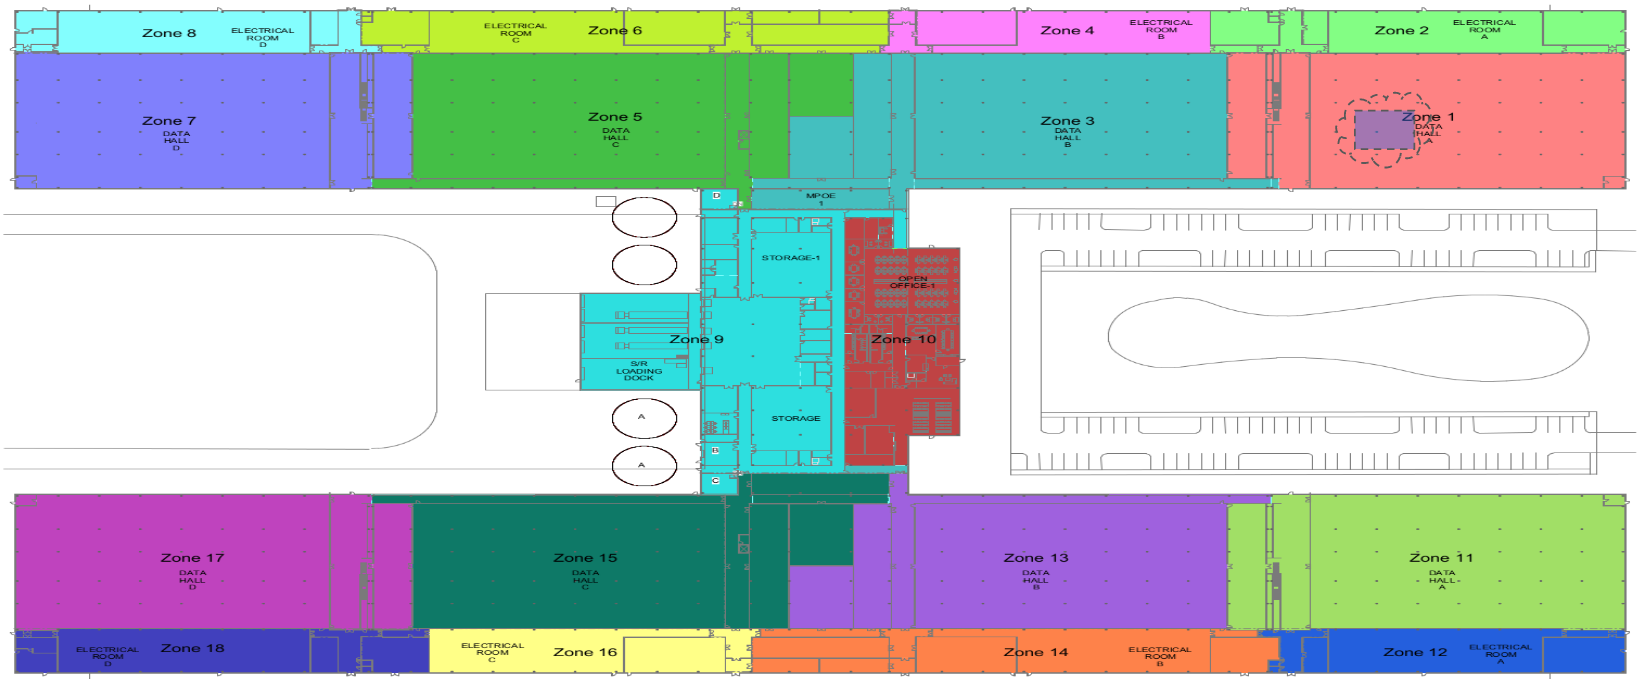
\includegraphics[scale=0.38]{conclusion/img/8_suite_80MW_dc.png}
    \caption[Scaling Data Center Facilites]{Relative Scale of Data Center Facilities compared to the EnergyPlus model used (confidential owner).}
    \label{system_boundary}
    % \end{figure}
\end{sidewaysfigure}

\subsection{Status Quo}
Over the last decade, there have been profound improvements in the energy efficiency of data centers. The US Department of Energy summarizes the operational improvements that have led to these improvements in Shehabi's 2016 report \cite{Shehabi16}. However, the rapid improvements also come with a cost of adapting new technology; for both building systems and IT hardware. Modeling these costs is not a trivial task given the breadth of the data center systems, where several generations of technologies may co-exist in the same platform. Nonetheless, business decisions around platform placement need to be based on global costs models. 

\subsection{Description of Gap}
To make global cost evaluations for a service platform, the inter-relationship between all of their physical resources need to be considered. For large platforms the data center costs are one of the most dominant expenditures. Within these data centers, there are three integrally coupled technical domains that influence the the costs; namely building systems, IT hardware equipment, and the operational costs. In the current practice most cost modeling is typically done for each domain in isolation from one another. One exception of this is in the building design phase where the building system design and operational energy are considered together. However, as discussed in Chapter~\ref{chp:bem} during the building design time - workload profiles are typically not known. 

In the current practice system cost models are done strictly from the bottoms-up. It is the bottoms-up approach that leads to the facility, its IT hardware, and operational costs to being evaluated in isolation from one another and then aggregated at the global level. In realty this is a very naive approach, as the nature of globally distributed services requires coordination across all of the facilities that the platform is deployed at. For example the need for data consistency requires that a user change of data in one country  propagates to data centers all over the world. With the inter-dependency there is a need for a modeling framework that can provide a global view of the platform operations from the top down while leveraging the granular insight that the bottoms up approach provide. 

\subsection{Contribution}
This dissertation contributes a four module framework that's capable of quantifying the global level costs for a network of data centers leaning on my experiences at four major internet platforms. Namely, the contributions of this work are presented in the form of software modules that can be implemented completely with open source software (ie EnergyPlus, Python). The underlying structure of this research are listed below.

\begin{enumerate}
    \item Candid description of data center design, deployment, and operations perspectives from hyper-scale data center experiences. 
    \item Building level energy model with load reset.
    \item Marginal costs of energy for data center that goes beyond renewable energy credits.
    \item A method to assess environmental costs using EEIO on a global network of data centers.
    \item Culmination of the thrcharactierisingee individual contribution into a singular framework.
\end{enumerate} 

By using the proposed framework a more representative end to end costs of data centers can be assessed. In the dissertation, in-lieu of monetary costs the system costs in terms of its carbon footprint are addressed. The framework also lends itself for monetary costs in industrial applications where real costs are obtainable.

\section{Summary of Finding}
\begin{enumerate}
    \item Cluster level abstraction suffices for building energy models - Chapter~\ref{chp:background}.
    \item Top down network modeling to understand geographical dependencies of the network of data centers. This is crucial to understand coincident energy supply and demand. Chapter~\ref{chp:mec}.
    \item Couple openly available EnergyPlus with external interfaces to characterize the IT load. \ref{chp:bem}
    \item Using a hybrid life cycle assessment method with EEIO based and process based apporaches can characterise a network of DCs. Chapter~\ref{chp:embodied_cost_model}.
\end{enumerate}


\subsection{Operational Carbon Footprint}
Table~\ref{dc_carbon_footprint} is illustrated in \ref{stacked_langs_at_dcs}.
\begin{figure}[h!]\centering
    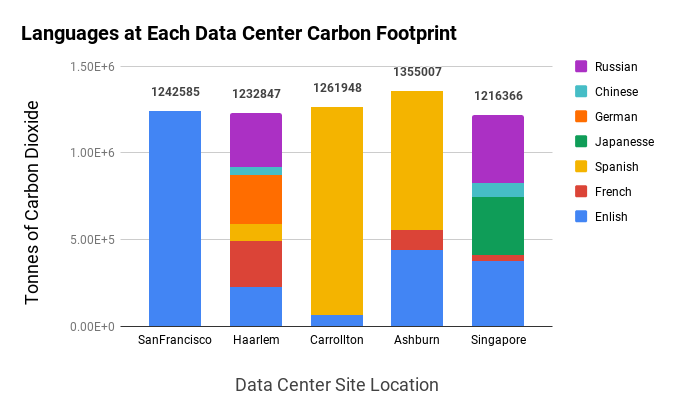
\includegraphics[scale=0.5]{embodied_cost_model/images/Languages at Each Data Center Carbon Footprint.png}
    \caption[Language to Data Center Carbon Footprint]{Language to Data Center Carbon Footprint.}
    \label{fig: land_dc_carbon}
\end{figure}



In reference to the functional unit of 1-kW of provisioned capacity the operation energy requirement for each DC-language pair is provide in \ref{functional_unit_bar}.

\begin{table}[h!]
    \begin{center}
    \scalebox{1.0}{
    \pgfplotstabletypeset[
        col sep=comma,
        string type,
        columns/Site/.style={column type={|l}},
        columns/en/.style={column type={|c}},
        columns/fr/.style={column type={|c}},
        columns/es/.style={column type={|c}},
        columns/ja/.style={column type={|c}},
        columns/de/.style={column type={|c}},
        columns/zh/.style={column type={|c}},
        columns/ru/.style={column type={|c|}},
        every head row/.style={before row=\hline,after row=\hline},
        every last row/.style={after row=\hline},
        every even row/.style={
            before row={\rowcolor[gray]{0.9}}},
        ]{embodied_cost_model/contents/data/functional_unit_matrix.csv}}
    \end{center}
    \caption[Operational Energy's $CO_2$ emissions per functional unit Matrix]{Operational energy's $CO_2$ emissions per functional unit matrix. For each Site (row) and Language (column) pair, the $CO_2$ density (tonnes) per provisioned kW data center capacity. Units: $CO_2$-tonnes per kW per year}
    \label{functional_unit_bar}
\end{table}

\section{Conclusions}
For DC global systems a model characterising the full system must span across IT and building domains. Characterize the usage profiles and their dependencies on the various types of physical resources. Accurately and similarly represent each data center a network within building energy models that are aware of the dynamic loads in the building - align coincident energy production, weather, and workloads.

TBC......

\section{Limitations}
The work has demonstrated the feasibility of coupling a global data center network across technology domains using information that are publicly shareable. The method and framework is technically sound, but the rapid change in technology supporting the industry and the various proprietary implementation of hardware designs, building architectures, and global network architecture necessitates that users of this framework characterise their own system's from the bottoms up first. Then, in lieu of naively summing up the bottoms-up values they use the demonstrated framework to evaluate the systems costs. One example benefit of this approach is that it will allow designers and operators to model their systems by changing simply changing a global level network policy (i.e. route less traffic to one facility and more to another).

One desired feature of the external coupling of the IT load is that it hides the complexity of the network model from the EnergyPlus implementation. In this work the network model is used to approximate the workloads, however more sophisticated models can also be used. Examples of more sophisticated models are adding the specific type of traffic (i.e. searching for a landmark vs. updating a landmark). This level of characterization is certainly out of the scope of BEM tools like EnergyPlus, so correlation factors must be externally developed and validated. The research in this work validated the workflow of the model, however its results were not validated against any real world DC operations. 


\section{Future Work}
\subsection{Capacity and Constraints Management}
Chapter~\ref{chp:bem} provides a discussion on using the proposed BEM to dynamically reset the capacity constrain values for DC. As discussed there, the DC are a building class where its utility is measures on the power delivered to and used by the IT equipment. Opportunistic allocation of power to IT equipment has tremendous values so pragmatically coupling this framework with cluster management software can yield 'free capacity' beyond the provisioned power capacity. The proposed framework not only makes the cluster management system aware of the real time capacity, it also supports scheduling decisions based on future load profiles. Furthermore, the workload scheduling component of the cluster management system can be made more robust with day ahead extensions to the module presented in Chapter \ref{chp:mec} to provide future energy costs or renewable capacity.


\subsection{Optimal Control}
In addition to increasing the supportable capacity of a DC, a IT load aware physics based energy model such as EnergyPlus can be used to optimize the real-time operations for the facility with the application of reinforcement learning techniques. The baseline for the model presented in Chapter~\ref{chp:bem}, GymEplus, is a demonstration of such an optimized control system. While GymEplus was not targeted towards data centers, it is easy to see how the model presented in this work can lend it left to GymEplus and only add one additional state variable to the reinforcement learning environment. Going even beyond the building control optimization present by GymEplus, a reinforcement learning agent can enable traffic load balancing amongst the set of DC based on arbitrary objective function that are aware of the state of the DC characterized by the presented modules. 



